\section{Zielsetzung}
\label{sec:Ziel}
Ziel des Versuches ist es mithilfe des Kugelfall-Viskosimeters nach Höppler die temperaturabhängige dynamische Viskosität $\eta(T)$ 
von destilliertem Wasser zu bestimmen. Es wird außerdem die Reynoldszahl bestimmt, um zu überprüfen wie turbulent die Strömung von
destilliertem Wasser ist.

\section{Theorie}
\label{sec:Theorie}

Bewegt sich ein Körper durch ein Material (gasförmig oder flüssig) so wirkt auf diesen eine Reibungskraft $\vec F_{\text{R}}$ entgegen der
Bewegungsrichtung, die von der Berührungsfläche des Körpers mit dem Material $A$ und der Geschwindigkeit des Körpers $\vec v$ abhängt.
Neben der Reibungskraft wirkt außerdem die Auftriebskraft $\vec F_{\text{A}}$ nach oben und die Schwerkraft $\vec F_{\text{G}}$ nach unten.
\newline Mithilfe des Stokes'schen Gesetzes lässt sich ein Zusammenhang zwischen der Reibungskraft und dem Körper herstellen. Die Relation ergibt
sich für eine Kugel zur Stokes'schen Reibungskraft (\ref{eqn:stokesR}) mit
\begin{align}
    \vec F_{\text{R}} = 6\pi\eta\vec v r.
    \label{eqn:stokesR}
\end{align}

Dabei steht das $r$ für den Radius der Kugel. Das $\eta$ ist eine temperaturabhängige Materialkonstante, die sich mithilfe der
Apparaturkonstanten $K$ durch die Formeln
\begin{align}
    \label{eqn:visko}
    \eta &= K (\rho_{K} - \rho_{\text{Fl}}) \cdot t, \\
    \label{eqn:andradescheGl}
    \eta(T) &= A\cdot\ln\Big(\frac{B}{T} \Big),
\end{align}
beschreiben lassen. \newline
Mithilfe von Gleichung (\ref{eqn:visko}) lässt sich die Viskosität , also die Zähigkeit ,eines Materials beim Kugelfallviskosimeter
bestimmen. Dabei ist das $K$ eine Apparaturkonstante, die die Kugelgeometrie und die Fallhöhe berücksichtigt.
$\rho_{K}$  ist die Dichte der Kugel und $\rho_{\text{Fl}}$ die Dichte des Materials, hier das einer Flüssigkeit. \newline
Gleichung (\ref{eqn:andradescheGl}) wird als \textit{Andradesche Gleichung} bezeichnet und beschreibt die Viskosität in Abhängigkeit 
von der Temperatur. $A$ und $B$ sind Konstanten, die sich durch (\ref{eqn:visko}) herleiten lassen.

Die Stokes'sche Reibungskraft $\vec F_{\text{R}}$ ist nur für laminare, nicht-turbulente, Strömungen gültig. Eine Aussage
über die Laminarität gibt die Reynoldszahl $Re$, die durch die folgende Gleichung (\ref{eqn:reynold}) beschrieben wird
\begin{align}
    \label{eqn:reynold}
    Re \coloneq \frac{\rho_{\text{Fl}} \vec v d}{\eta}.
\end{align}
Dabei bezeichnet $d$ den Durchmesser des Fallrohres eines Viskosimeters, was in \autoref{subsec:viskosm} beschrieben wird.

Die Dichte einer Kugel wird durch
\begin{align}
    \label{eqn:vKugel}
    \rho_{\text{K}} = \frac{M}{V} = \frac{4\cdot M}{3\pi r^3}
\end{align}
berechnet.

\subsection{Kugelfall-Viskosimeter nach Höppler}
\label{subsec:viskosm}
Für das Experiment wird ein Kugelfallviskosimeter nach Höppler, wie in \autoref{Abb:viskosimeter} verwendet.

\begin{figure}
    \centering
    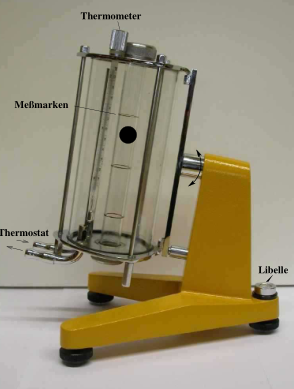
\includegraphics[width=5.5cm]{Dateien/Viskosimeter.png}
    \caption{Im Experiment verwendetes Viskosimeter \cite{anleitung107}.}
    \label{Abb:viskosimeter}
\end{figure}

Das Viskosimeter besteht aus einem Fallrohr, das sich in einem mit Wasserbad befindet, dessen Temperatur geregelt werden kann.
Das Fallrohr besitzt an beiden Öffnungen jeweils eine Öffnung, die es ermöglicht es mit einer zu untersuchenden Substanz und einer
Testkugel zu befüllen. Es ist außerdem leicht geneigt, um eine möglichst wirbelfreie, laminare Strömung zu erzeugen. 
An der Glaswand des Rohres befinden sich drei Markierungen, die jeweils $\SI{5}{\cm}$ auseinander liegen. Das Viskosimeter steht auf einem
Ständer mit drei höhenverstellbaren Füßen. Um es möglichst gerade auszurichten ist an einem der dreien eine Libelle angebracht.